
%https://de.wikipedia.org/wiki/Datei:Electronic_component_inductors.jpg

\begin{wrapfigure}[5]{r}[-1cm]{3cm}
 \vspace{-5cm}
 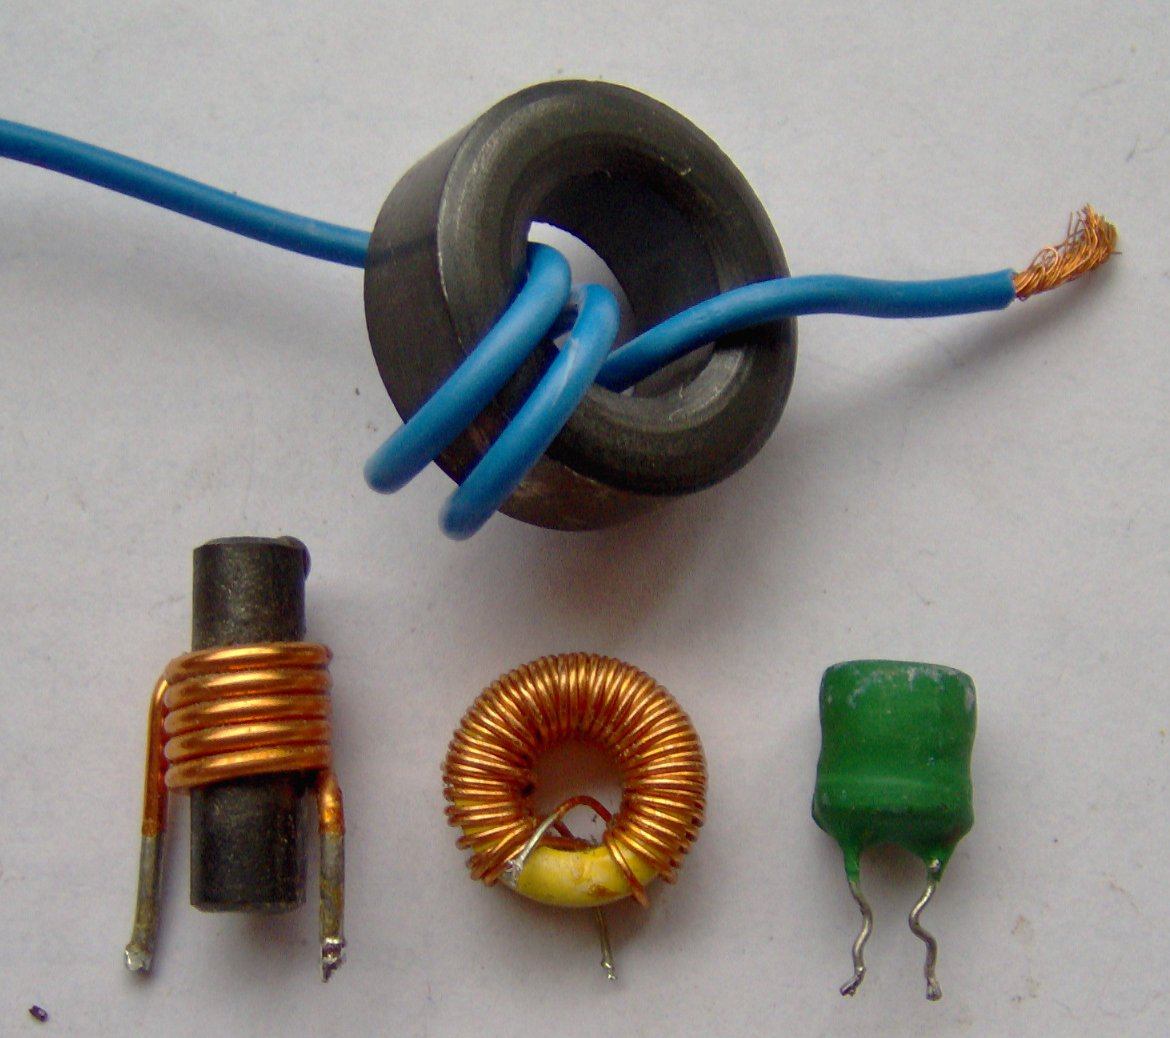
\includegraphics[scale=0.1]{Spule/Bilder/Electronic_component_inductors.jpg}
 \vspace{-5cm}
\end{wrapfigure}

\section*{Theorie- und Prüfungsfragen} 
~~~
\begin{enumerate}
\itemsep1pt\parskip0pt\parsep0pt
\item[1] Wie lässt sich die Induktivität einer Spule berechnen?
\item[2] Wie lautet die magnetische Feldkonstante $\mu_0$?
\item[3] Wie lautet die relative Permeabilität $\mu_r$ für Luft?
\item[4] Berechne die Induktivität der Zylinderspule mit folgender Bemaßung: 25 Windungen, 	Durchmesser von 8mm, Länge 1cm, relative Permeabilität von Luft
\end{enumerate}



%\begin{block}
\aufgabentext{
	\begin{enumerate}
	\item[5] \emph{\textbf{TB402}}  Wie nennt man das Feld im Innern einer langen Zylinderspule beim Fließen eines Gleichstroms?
		\begin{enumerate}
		\itemsep1pt\parskip0pt\parsep0pt
		\item[A] Homogenes elektrisches Feld
		\item[B] Zentriertes magnetisches Feld
		\item[C] Konzentrisches Magnetfeld
		\item[D] Homogenes magnetisches Feld 
		\loesung{D}
		\end{enumerate}
	\end{enumerate}
}
%\end{block}

%\begin{block}
\aufgabentext{
	\begin{enumerate}
	\item[6] \emph{\textbf{TC302}} Wie ändert sich die Induktivität einer Spule von $12 \mu H$, wenn die Wicklung auf dem Wickelkörper bei gleicher Windungszahl auf den doppelten Wert auseinander gezogen wird?
		\begin{enumerate}
		\itemsep1pt\parskip0pt\parsep0pt
			\item[A] Die Induktivität sinkt auf $3 \mu H$.
			\item[B] Die Induktivität sinkt auf $6 \mu H$. 
			\item[C]  Die Induktivität steigt auf $24 \mu H$.
			\item[D] Die Induktivität steigt auf $48 \mu H$.
			\loesung{B}
		\end{enumerate}	
	\end{enumerate}	
%\end{block}
}
%\begin{block}
\aufgabentext{
	\begin{enumerate}
		\item[7] \emph{\textbf{TC303}} Wie kann man die Induktivität einer Spule vergrößern?
		\begin{enumerate}
		\itemsep1pt\parskip0pt\parsep0pt
			\item[A]  Durch Auseinanderziehen der Spule (Vergrößerung der Spulenlänge).
			\item[B] Durch Einführen eines Kupferkerns in die Spule.
			\item[C] Durch Stauchen der Spule (Verkürzen der Spulenlänge). 
			\item[D] Durch Einbau der Spule in einen Abschirmbecher.
			\loesung{C}
		\end{enumerate}
	\end{enumerate}
%\end{block}
}

\loesung{
	\begin{align}
	i) ~& L ~&=&~ & \dfrac{\mu_0 \cdot \mu_r \cdot A \cdot N^2}{l}\\
	ii) ~& \mu_0 ~&=&~ & 1,2566\cdot 10^{-6} \frac{H}{m}\\
	iii) ~& \mu_{r, Luft} ~& = &~ & 1 + 4 \cdot 10^{-7}\\
	iv) ~& L ~&=&~& 3,9\mu H
	\end{align}
	}


%----------------------------
\newpage

\section*{Praktische Anwendung}

\subsection*{Spule wickeln}

\begin{wrapfigure}{r}{0.4\textwidth}
 \vspace{-10pt}
 \centering 
 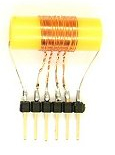
\includegraphics[scale=4]{Spule/Bilder/Spule_bau.jpg}
 %\caption{Bildunterschrift der Grafik.}
 %\label{fig:meine-Grafik}
 \vspace{-5pt}
\end{wrapfigure}

Für den ersten Versuch soll eine Spule mit insgesamt $25 $Windungen und vier Anzapfungen gewickelt werden. Als Wickelkörper soll eine 8 mm dickes und $3cm$ langes Stück eines Trinkhalmes verwendet werden. Zwei Löcher im Abstand $1cm$ helfen die Drahtenden zu fixieren. Es werden dann jeweils $5$ Windungen gewickelt, eine Schlaufe verdrillt und die folgenden Windungen aufgetragen. Die fertige Spule wird an einen Abschnitt Pfostenstecker mit sechs Kontakten gelötet. 

